
\documentclass[12pt, oneside]{amsart}
\usepackage[font={sf}]{caption}
\usepackage[]{graphics}
\usepackage{graphicx}
\usepackage{epstopdf}
\usepackage{hyperref}
\hypersetup{breaklinks=true, colorlinks=true, citecolor=blue}
\usepackage{natbib}
\usepackage{color}
\usepackage{soul}
\usepackage{rotating}
\usepackage{tabularx}
\usepackage{longtable}
\usepackage{lscape}
\usepackage{array}
\usepackage{multirow}
\usepackage{setspace}
\usepackage{textcomp}
\usepackage{dcolumn}
\setlength{\LTcapwidth}{6in}
\usepackage{dcolumn}
\usepackage[margin=1in]{geometry}

 \bibpunct{(}{)}{,}{a}{}{,}
 \doublespacing
 \raggedright
 \setlength{\parindent}{15pt} 


\begin{document}
%\setcounter{secnumdepth}{0}


{ \Large \bf Figures}


%\tableofcontents
%\listoftables
%\renewcommand\thesection{S1}
%\listoffigures

\begin{figure}[h]
\begin{center}
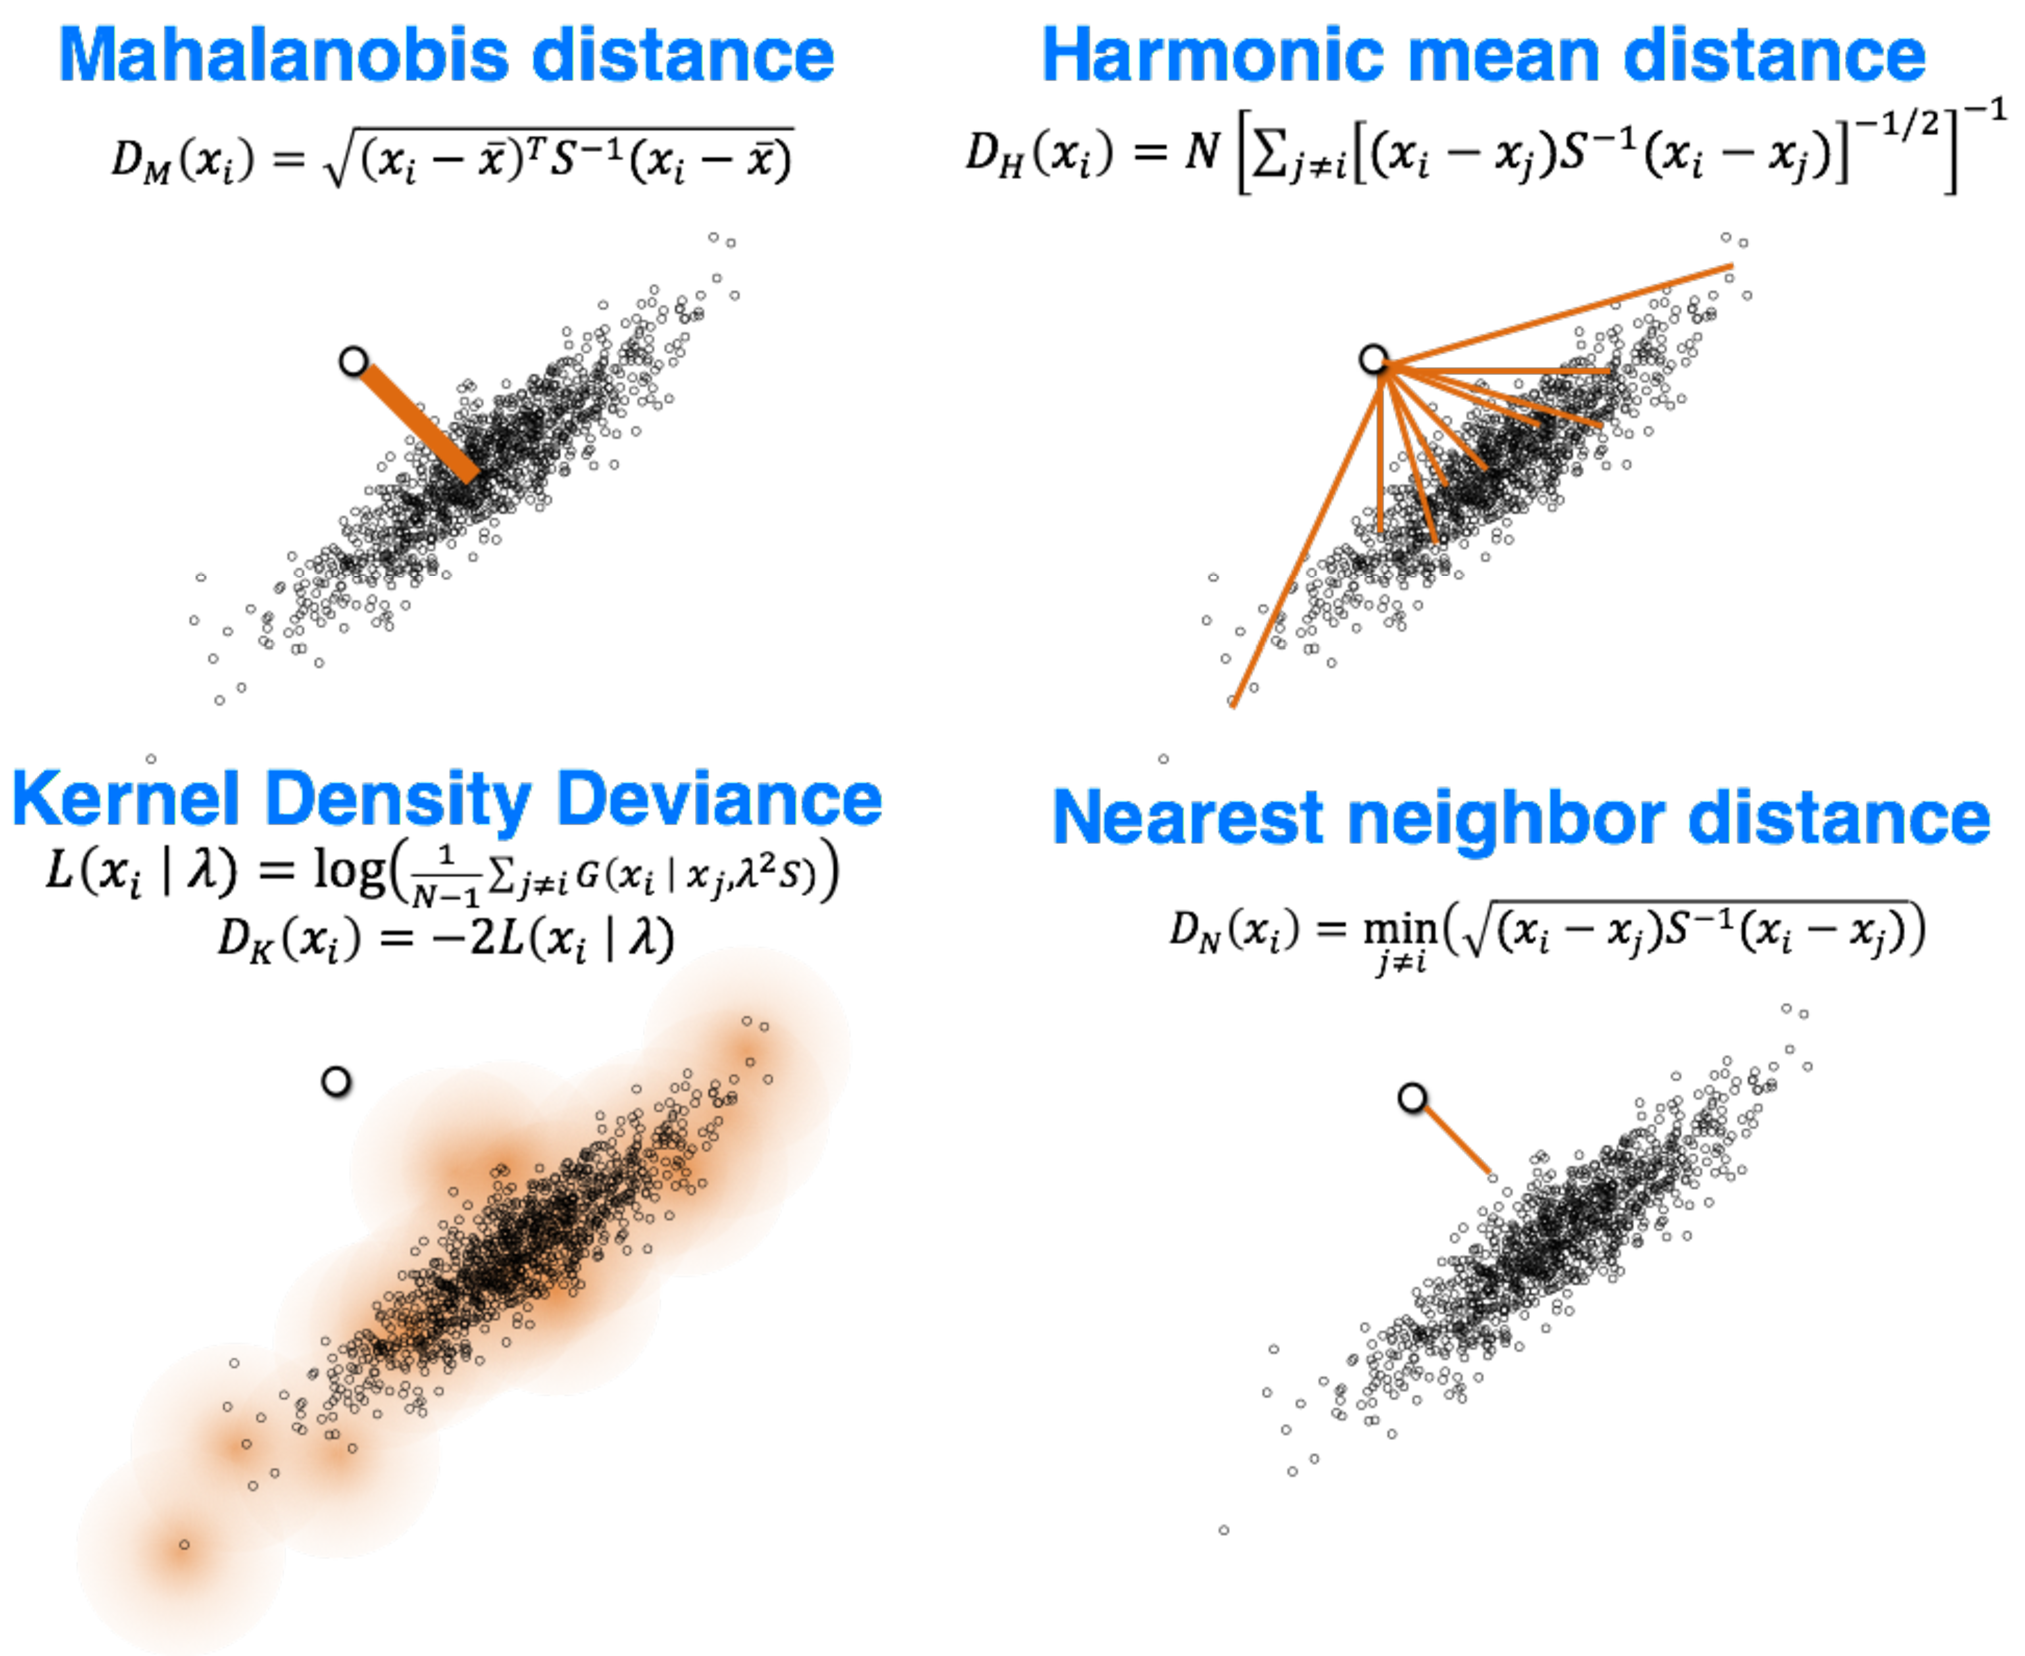
\includegraphics[width=6in]{../figures_man2/F1-FourMeasures.pdf}
\end{center}
\caption[]{Conceptual examples of the four multivariate statistics compared in this study. 

{\bf TO DO: Add ABCD.

TEAM: Would anyone like to take on making a figure like this one, but better for publication? I made these in power point, which is why they are awful. I think the kernel deviance could be challenging to visualize, because technically the bandwidth should be proportional to the variance in each dimension. The harmonic mean could also be challenging, because that is a lot of overlapping lines to draw. It might be good to draw the lines first with transparency=0.1 and lay the points on top.}} 
 \label{fig:???}
\end{figure}

\newpage
\begin{figure}[h]
\begin{center}
\includegraphics[width=6in]{../figures_man2/F4-LandsharcSummary.pdf}
\end{center}
\caption[]{Comparison of univariate and multivariate statistics for their power to separate signals of selection from neutrality. Each row represents one of the simulated demographies (IM = Island Model, IBD = Isolation By Distance, 1R = range expansion from one refuge, 2R = range expansion from two refugia). The four univariate statistics (grey box plots) evaluated were: $X^TX$ (xtx), Bayes Factors (bf), Spearman's $\rho$, and  $Z$-scores (lfmm).} 
 \label{fig:???}
\end{figure}

\newpage
\begin{figure}[h]
\begin{center}
\includegraphics[width=4in]{../figures_man2/F2-LandsharcCompareToNeutralCovMat.pdf}
\end{center}
\caption[]{Comparison of the mean absolute difference between the variance-covariance matrix among the univariate statistics calculated using (i) all the data, (ii) the MCD estimate using 75\% of the dataset, and (iii) the MCD estimate using 99\% of the dataset.  Boxplots are summarized over all demographies and sampling designs.

{\bf TO DO: Should I switch MCD99 and MCD75 here, since MCD99 will be closer to "all data" than MCD75?}
} 
 \label{fig:???}
\end{figure}

\newpage
\begin{figure}[h]
\begin{center}
\includegraphics[width=6in]{../figures_man2/F1-CovEllipse_4NeutralMCDpoints.png}
\end{center}
\caption[]{Comparison of 99\% confidence intervals on the two dimensional ellipse given by the determinant on the covariance matrix between these two variables calculated from: (i) all the data, (ii) neutral loci only, and (iii) the MCD estimate. 

{\bf TEAM: does this visualize that the robust points are neutral or is it unclear?

TO DO: Need to add legend to this plot (neutral = grey, trianges = different strengths of selection, pink dots = robust points).  Replace "xtx" with $X^TX$ and rho with Spearman's $\rho$. Maybe change the colors so that neutral ellipse is black, and change the lines so that it works in BW.
}
}
 \label{fig:???}
\end{figure}



\newpage
\begin{figure}[h]
\begin{center}
\includegraphics[height=6in]{../figures_man2/F3-LandsharcProportionSelectedMCD.pdf}
\end{center}
\caption[]{Evaluation of whether loci affected by selection were identified as 'robust' points (e.g., not outliers) by the MCD algorithm. Loci under relatively weak selection (s=0.005) are in the left column, well loci under moderate selection are in the right column (s=0.01). The horizontal dashed line represents the null expectation, based on the proportion of loci under that strength of selection in the entire dataset. The MCD never identified loci simulated under strong selection (s=0.1) as robust (expected = 0.001 in IBD and 0.0017 in IM, 1R, and 2R; observed = 0 across all simulations).} 
 \label{fig:???}
\end{figure}



\newpage
\begin{figure}[h]
\begin{center}
\includegraphics[width=4in]{../figures_man2/F5-LandsharcFalsePositivesMCD.pdf}
\end{center}
\caption[]{The number of false discoveries (neutral loci inferred to be outliers, out of 9900 total neutral loci in the dataset) resulting if robust points identified by the MCD are used as an empirical null distribution.} 
 \label{fig:???}
\end{figure}

\end{document}